\documentclass{beamer}
\usepackage{listings}
\lstset{
%language=C,
frame=single, 
breaklines=true,
columns=fullflexible
}
\usepackage{blkarray}
\usepackage{subcaption}
\usepackage{url}
\usepackage{xurl}
\usepackage{tikz}
\usepackage{tkz-euclide} % loads  TikZ and tkz-base
%\usetkzobj{all}
\usetikzlibrary{calc,math}
\usepackage{float}
\newcommand\norm[1]{\left\lVert#1\right\rVert}
\renewcommand{\vec}[1]{\mathbf{#1}}
\usepackage[export]{adjustbox}
\usepackage[utf8]{inputenc}
\usepackage{amsmath}
\usepackage{amssymb}
\usepackage{bm}
\usepackage{tikz}
\usetikzlibrary{automata, positioning}
\usetheme{Boadilla}
\providecommand{\pr}[1]{\ensuremath{\Pr\left(#1\right)}}
\providecommand{\sbrak}[1]{\ensuremath{{}\left[#1\right]}}
\providecommand{\lsbrak}[1]{\ensuremath{{}\left[#1\right.}}
\providecommand{\rsbrak}[1]{\ensuremath{{}\left.#1\right]}}
\providecommand{\pr}[1]{\ensuremath{\Pr\left(#1\right)}}
\providecommand{\brak}[1]{\ensuremath{\left(#1\right)}}
\providecommand{\lbrak}[1]{\ensuremath{\left(#1\right.}}
\providecommand{\rbrak}[1]{\ensuremath{\left.#1\right)}}
\providecommand{\cbrak}[1]{\ensuremath{\left\{#1\right\}}}
\providecommand{\lcbrak}[1]{\ensuremath{\left\{#1\right.}}
\providecommand{\rcbrak}[1]{\ensuremath{\left.#1\right\}}}

\title{Research paper presentation}
\author{Yashas Tadikamalla}
\date{AI20BTECH11027}
\begin{document}

\begin{frame}
\titlepage
\end{frame}

\begin{frame}
    \begin{block}{Title}
    A Maximum-Likelihood TDOA Localization Algorithm Using Difference-of-Convex Programming.
    \end{block}
    \begin{block}{Authors}
    \begin{itemize}
        \item Xiuxiu Ma, Tarig Ballal, Member, IEEE
        \item Hui Chen, Student Member, IEEE
        \item Omar Aldayel, Member, IEEE
        \item Tareq Y. Al-Naffouri, Senior Member, IEEE
    \end{itemize}
    \end{block}
    \begin{block}{Date of publication}
    January 14, 2021.
    \end{block}
\end{frame}

\begin{frame}
\frametitle{}
\begin{block}{Wireless sensor networks (WSN)}
WSN refers to a group of spatially dispersed and dedicated sensors for monitoring and recording the physical conditions of the environment. They are widely used for military, commercial purposes.
\end{block}
\begin{block}{Source localization}
Source localization is the key problem in WSN, navigation, etc. It refers to finding of the unknown location of a source node, using the noisy measurements from the nodes in known locations, called the anchor nodes. 
\end{block}
\begin{block}{Localization techniques}
\begin{enumerate}
    \item Angle of Arrival (AoA)
    \item Time of Arrival (ToA)
    \item Time Difference of Arrival (TDoA), etc.
\end{enumerate} 
\end{block}

\end{frame}

\begin{frame}
\frametitle{}
\begin{block}{Convex set}
A set is said to be convex if, the line segment joining any two points in it, is contained completely within the set.
\begin{figure}[h!]
\centering
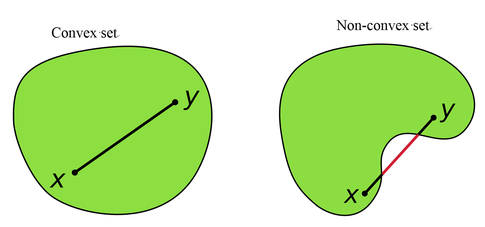
\includegraphics[scale=0.2]{fig1.png}
\caption{Convex and non convex sets}
\label{ex}
\end{figure}
\end{block}
\begin{block}{Convex hull}
The convex hull of a given set $X$ may be defined as the intersection of all convex sets containing $X$.
\begin{figure}[h!]
\centering
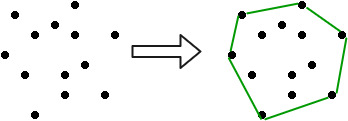
\includegraphics[scale=0.3]{fig3.jpg}
\caption{Convex Hull}
\label{ex}
\end{figure}
\end{block}
\end{frame}

\begin{frame}
\frametitle{}
\begin{block}{Convex and Concave functions}
A real valued function defined on an $n$ dimensional interval, is said to be convex, if the line segment between any two points on the graph of the function lies above the graph between the two points. A concave function can be defined as the negative of a convex function.
\begin{figure}
    \centering
    \begin{subfigure}[b!]{0.45\linewidth}
    \centering
    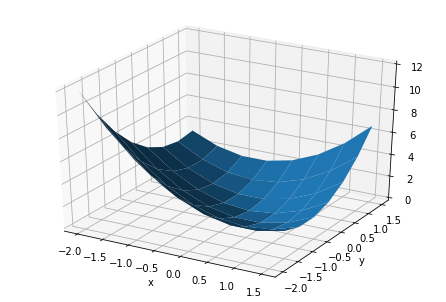
\includegraphics[scale=0.35]{fig21.png}
    \caption{Bivariate convex function $x^{2}+xy+y^{2}$} 
    \label{fig:img21}
    \end{subfigure}
    \begin{subfigure}[b!]{0.45\linewidth}
    \centering
    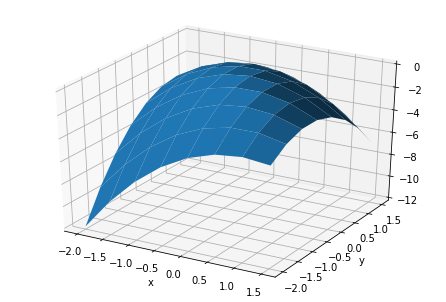
\includegraphics[scale=0.35]{fig22.png}
    \caption{Bivariate concave function $-(x^{2}+xy+y^{2})$}
    \label{fig:img22}
    \end{subfigure}
\end{figure}
\end{block}
\end{frame}

\begin{frame}
\frametitle{}
\begin{block}{Maximum Likelihood (ML) concept}
ML is a method used to find parameter values for a model describing certain process, such that, the likelihood of the model is maximised, i.e, the data produced by it, is as close as possible to the actual data.
%We need it to minimize the deviation between the actual and estimated positions.
\end{block}
\begin{block}{Difference-of-Convex (DC) programming}
The optimization of an objective function on a convex set is called DC programming, if it can be represented as difference of convex functions.
\end{block}
\begin{block}{Convex-Concave procedure (CCCP)}
CCCP is a DC programming tool for finding a local optimum.
\end{block}
\begin{block}{Cramér-Rao Lower bound (CRLB)}
In estimation theory and statistics, the CRLB expresses a lower bound on the variance of unbiased estimators. An unbiased estimator which achieves this lower bound is said to be fully efficient.
\end{block}
\end{frame}

\begin{frame}
\frametitle{Abstract}
\begin{block}{}
\begin{enumerate}
    \item We can use TDOA measurements to construct an objective function based on the ML method to estimate a source location. This objective function needs to be minimised.
    \item The difficulty in this optimization process is the non-convexity of the objective function, which precludes the use of many standard convex optimization tools. Usually, approximations such as convex relaxation, when applied, result in performance loss.
    \item So, we employ DC programming tools, by modifying the objective function into an exact difference of two convex functions. This guarantees convergence of the objective function to a stationary point.
    \item Simulation results show that, when initialized within the convex hull of the anchors, the proposed TDOA localization algorithm outperforms a number of benchmark methods, behaves as an exact ML estimator, and indeed achieves the CRLB.
\end{enumerate}
\end{block}
\end{frame}

\begin{frame}
\frametitle{Problem Formulation : Objective Function based on ML}
Consider a system consisting of $N$ anchors installed at known positions $\bm{r}_{i}, i=1,2,\dots N$. These anchors collaborate to localize an unknown source located at $\bm{p}$. For any signal emitted by the source, the time difference of arrival (TDOA) observed between two anchors at $\bm{r}_{i}$ and $\bm{r}_{j}$ is given by
\begin{align}
\label{eq:1}
    \tau_{ij}(\bm{p})=\dfrac{1}{v}(\|\bm{p}-\bm{r}_{i}\|_{2}-\|\bm{p}-\bm{r}_{j}\|_{2})
\end{align}
where v is the signal propagation speed, and $\|.\|_{2}$ denotes the $l_{2}$ norm. In practice, the actual TDOA values are unknown, only measurements of the form $\widehat{\tau_{ij}}=\tau_{ij}(\bm{p})+n_{ij}$ are available, where $n_{ij}$ is additive noise. Assuming that the additive noise terms $n_{ij}$ are i.i.d. Gaussian, ML estimation of the source location boils down to the minimization
\begin{align}
    \widehat{\bm{p}}=\text{arg}\min_{\bm{p}} c(\bm{p})=\text{arg}\min_{\bm{p}}\displaystyle \sum_{i\neq j}\sbrak{\widehat{\tau_{ij}}-\tau_{ij}(\bm{p})}^{2}
\end{align}
\end{frame}

\begin{frame}
\frametitle{Problem formulation : Objective Function based on ML}
The objective function $c(\bm{p})$ can be expanded as
\begin{align}
    c(\bm{p})=2\displaystyle \sum_{i\neq j}c_{ij}(\bm{p})=2\displaystyle \sum_{i\neq j}\sbrak{f_{ij}(\bm{p})-g_{ij}(\bm{p})-q_{ij}(\bm{p})}
\end{align}
where,
\begin{align}
    f_{ij}(\bm{p})=\dfrac{\widehat{\tau_{ij}}^{2}}{2}+\dfrac{1}{2v^{2}}\|\bm{p}-\bm{r}_{i}\|_{2}^{2}+\dfrac{1}{2v^{2}}\|\bm{p}-\bm{r}_{j}\|_{2}^{2}\\
    g_{ij}(\bm{p})=\dfrac{1}{v^{2}}\|\bm{p}-\bm{r}_{i}\|_{2}\|\bm{p}-\bm{r}_{j}\|_{2}\\
    q_{ij}(\bm{p})=\dfrac{\widehat{\tau_{ij}}}{v}(\|\bm{p}-\bm{r}_{i}\|_{2}-\|\bm{p}-\bm{r}_{j}\|_{2})
\end{align}
\end{frame}
 
\begin{frame}
\frametitle{Problem formulation : Objective Function based on ML}
It can be seen that $f_{ij}(\bm{p})$ is convex, $g_{ij}(\bm{p})$, $q_{ij}(\bm{p})$ are non convex. (As they respectively consist of norm products and norm differences). 
\begin{figure}
    \centering
    \begin{subfigure}[b!]{0.45\linewidth}
    \centering
    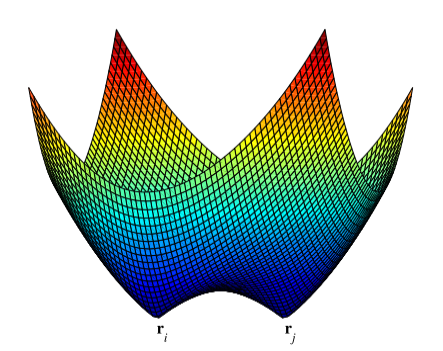
\includegraphics[scale=0.35]{fig4.png}
    \caption{An example plot of the non-convex component $g_{ij}(\bm{p})$} 
    \label{fig:img4}
    \end{subfigure}
    \begin{subfigure}[b!]{0.45\linewidth}
    \centering
    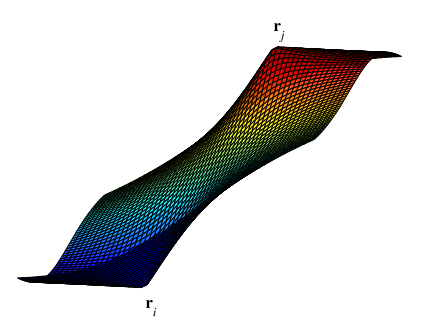
\includegraphics[scale=0.35]{fig5.png}
    \caption{An example plot of the non-convex component $q_{ij}(\bm{p})$ for a positive $\widehat{\tau_{ij}}$}
    \label{fig:img5}
    \end{subfigure}
\end{figure}
For a general case, $c(\bm{p})$ turns out to be a non convex function. Hence we cannot use the standard convex optimization tools. So, we try to use the DC programming approach.
\end{frame}

\begin{frame}
\frametitle{DC programming}
Let us construct two appropriate functions $\alpha_{ij}(\bm{p})$ and $\beta_{ij}(\bm{p})$, such that, $f_{ij}(\bm{p})-\alpha_{ij}(\bm{p})-\beta_{ij}(\bm{p}), g_{ij}(\bm{p})-\alpha_{ij}(\bm{p}), q_{ij}(\bm{p})-\beta_{ij}(\bm{p})$ are all convex functions. This allows us to convert $c_{ij}(\bm{p})$ as
\begin{align}
\label{eq:dc}
    c_{ij}(\bm{p})=c_{ij,1}(\bm{p})-c_{ij,2}(\bm{p})
\end{align}
where, 
\begin{align}
    &c_{ij,1}(\bm{p})=f_{ij}(\bm{p})-\alpha_{ij}(\bm{p})-\beta_{ij}(\bm{p}),\\
    &c_{ij,2}(\bm{p})=g_{ij}(\bm{p})-\alpha_{ij}(\bm{p})+q_{ij}(\bm{p})-\beta_{ij}(\bm{p})
\end{align}
As for how to construct $\alpha_{ij}(\bm{p})$ and $\beta_{ij}(\bm{p})$, we just need to ensure that these functions are more concave than the most concave part of $g_{ij}(\bm{p})$ and $q_{ij}(\bm{p})$. 
\end{frame}

\begin{frame}
\frametitle{DC programming}
Specifically, we set,
\begin{align}
    &\alpha_{ij}(\bm{p})=-\dfrac{1}{v^{2}}(\bm{p}-r_{i})^{T}(\bm{p}-r_{j}),\\
    &\beta_{ij}(\bm{p})=-b\dfrac{\widehat{\tau_{ij}}}{v}\|\bm{p}-\bm{r}_{j}\|_{2}+(1-b)\dfrac{\widehat{\tau_{ij}}}{v}\|\bm{p}-\bm{r}_{i}\|_{2}
\end{align}
where $b=1$ for $\widehat{\tau_{ij}}\geq 0$, and $b=0$ for $\widehat{\tau_{ij}}< 0$.
\begin{align}
\label{eq:abc}
    &g_{ij}(\bm{p})-\alpha_{ij}(\bm{p})=\dfrac{1}{v^{2}}\sbrak{\|\bm{p}-\bm{r}_{i}\|_{2}\|\bm{p}-\bm{r}_{j}\|_{2}+(\bm{p}-r_{i})^{T}(\bm{p}-r_{j})}\\
\label{eq:xyz}
    &q_{ij}(\bm{p})-\beta_{ij}(\bm{p})=\begin{cases}
    \dfrac{\widehat{\tau_{ij}}}{v}\|\bm{p}-\bm{r}_{i}\|_{2}, & \widehat{\tau_{ij}}\geq 0 \\~\\[-1em]
	-\dfrac{\widehat{\tau_{ij}}}{v}\|\bm{p}-\bm{r}_{j}\|_{2}, & \widehat{\tau_{ij}}<0
    \end{cases}
\end{align}
\end{frame}

\begin{frame}
\frametitle{DC programming}
\begin{block}{Proof for $g_{ij}(\bm{p})-\alpha_{ij}(\bm{p})$ being convex}
\url{https://github.com/gadepall/papers/blob/master/Research-papers/sp2.pdf}
\end{block}
\begin{block}{Proof for $q_{ij}(\bm{p})-\beta_{ij}(\bm{p})$ being convex, regardless of $\widehat{\tau_{ij}}$}
As $q_{ij}(\bm{p})-\beta_{ij}(\bm{p})$ is non negative $l_{2}$ norm,$\forall \widehat{\tau_{ij}}$, it is convex.
\end{block}
Hence, $c_{ij,1}(\bm{p}),c_{ij,2}(\bm{p})$ are convex. Therefore, \eqref{eq:dc} is a DC function.
\end{frame}

\begin{frame} 
\frametitle{Iterative CCCP-ML algorithm} 
Let $E(\bm{p})=a(\bm{p})-b(\bm{p})$, be a continuous DC function over $D$. Consider an iterative algorithm that seeks to minimize $E(\bm{p})$. By definition, for any $\bm{p}_{1},\bm{p}_{2}\in D$,
\begin{align}
    \label{eq:one}
    &a(\bm{p}_{2})\leq a(\bm{p}_{1})-(\bm{p}_{1}-\bm{p}_{2})^{T}\nabla a(\bm{p}_{2})\\
    \label{eq:two}
    &-b(\bm{p}_{2})\leq -b(\bm{p}_{1})+(\bm{p}_{1}-\bm{p}_{2})^{T}\nabla (-b(\bm{p}_{2}))
\end{align}
where, $\nabla$ is the gradient operator. Let $\bm{p}^{t},\bm{p}^{t+1}$ are results of two consecutive iterations. By setting $\bm{p}_{1}=\bm{p}^{t},\bm{p}_{2}=\bm{p}^{t+1}$, and adding \eqref{eq:one}, \eqref{eq:two}
\begin{align}
\label{eq:wow}
    E(\bm{p}^{t+1})\leq E(\bm{p}^{t})+(\Delta \bm{p})^{T}(\nabla a(\bm{p}^{t+1})+ \nabla (-b(\bm{p}^{t})))
\end{align}
where, $\Delta\bm{p}=\bm{p}^{t+1}-\bm{p}^{t}$.  So,  
\begin{align}
\label{eq:cccp}
    \nabla a(\bm{p}^{t+1})+ \nabla (-b(\bm{p}^{t}))=0
\end{align}
is a sufficient condition for $E(\bm{p}^{t+1})\leq E(\bm{p}^{t})$. Hence, this iterative method guarantees convergence to a stationary point. 

\end{frame}

\begin{frame}
\frametitle{Iterative CCCP-ML algorithm}
Thus, the CCCP-ML algorithm applies \eqref{eq:cccp} as a rule to determine $\bm{p}^{t+1}$, given $\nabla b(\bm{p}^{t})$.
    \begin{enumerate}
    \item Initialize : $t=0,\bm{p}^{t}=\bm{p}^{0}$
    \item Repeat (CCCP/outer loop) :
    \begin{itemize}
        \item Compute : $g_{t}=\displaystyle \sum_{i\neq j}\nabla c_{ij,2}(\bm{p}^{t})$
        \item Compute (gradient/inner loop) : $\bm{p}^{t+1}=\text{arg}\min_{\bm{p}}\displaystyle \sum_{i\neq j}c_{ij,1}(\bm{p})-\bm{p}^{T}g_{t}$
        \item $t=t+1$
        \item  Quit when the value of the objective function is sufficiently small.
        \end{itemize}
\end{enumerate}
\end{frame}

\begin{frame} 
\frametitle{Note} 
\begin{itemize}
    \item The proposed method can be utilized for both 2D, 3D localization. To simplify the presentation of the results, we focus our simulations on 2D scenarios with different number of anchors, anchor placements and source locations.
    \item When the source is located outside the anchors’ convex hull, the objective function is flat near the source and remains so as we move away from the convex hull. This makes estimating the source location infeasible, regardless of the method applied.
    \item Therefore, we evaluate performance only in scenarios involving source locations inside the anchors’ convex hull. In such scenarios, it is observed that initialization outside the convex hull does not guarantee convergence to the correct solution.
    \item Therefore, we initialize the proposed method, and all the tested iterative methods, randomly within the convex hull.
\end{itemize}
\end{frame}

\begin{frame} 
\frametitle{Simulation results} 
\begin{itemize}
    \item For each simulation scenario, TDOA across different anchor pairs is calculated using \eqref{eq:1}. Independently distributed errors are then added to simulate practical TDOA measurements. The errors are generated as Gaussian noises with zero mean and a standard deviation $\sigma$.
    \item  Localization performance is evaluated using the root mean squared error (RMSE) calculated from $10^{3}$ independent trials for each $\sigma$ value.
    \item The proposed method is compared with the following benchmark methods : The convex relaxation SDP, The CCCP-SOCP method, The CCCP-LP method, The I2WLS method.
    \item The proposed algorithm outperforms all the benchmark methods in all scenarios, achieving or staying very close to the CRLB.
    \item The performance of all methods tends to deteriorate as TDOA noise levels increase. However, the benchmark methods exhibit greater performance deterioration compared to the proposed method. This makes the advantage of the proposed method more visible in scenarios with high noise levels.
    
\end{itemize}
\end{frame}

\begin{frame}
\frametitle{Simulation results}
    \begin{figure}
    \centering
    \begin{subfigure}[b!]{0.45\linewidth}
    \centering
    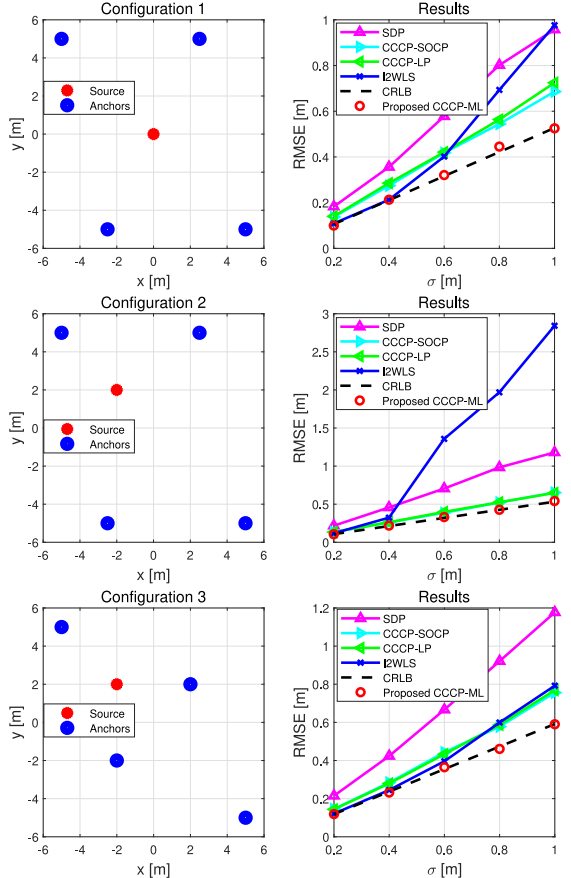
\includegraphics[scale=0.3]{fig61.png}
    \caption{Simulation results for the configuration with 4 anchors} 
    \label{fig:img61}
    \end{subfigure}
    \begin{subfigure}[b!]{0.45\linewidth}
    \centering
    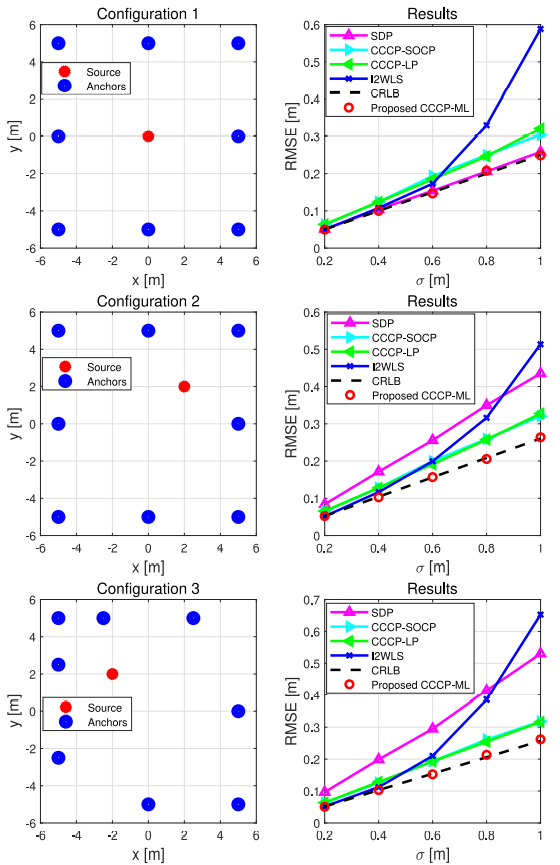
\includegraphics[scale=0.3]{fig62.png}
    \caption{Simulation results for the configuration with 8 anchors}
    \label{fig:img62}
    \end{subfigure}
\end{figure}
\end{frame}

\begin{frame}
\frametitle{Conclusion}
    \begin{itemize}
        \item We have presented a ML TDOA localization algorithm based on the CCCP. 
        \item We have shown that the ML TDOA localization problem can be posed as an exact difference-of-convex (DC) program by manipulating the ML objective function. Hence, the CCCP can be applied as an iterative method that guarantees convergence to a stationary point.
        \item  We have shown that, by initializing the proposed algorithm inside the anchors’ convex hull, the proposed CCCP-ML algorithm achieves the Cramér-Rao lower bound, hence outperforming a host of benchmark methods.

    \end{itemize}
\end{frame}

\end{document}